\section{Вычислительные эксперименты}

    \subsection{Алгоритм}
        Для компьютерного вычисления будем использовать метод Рунге-Кутты, с помощью которого получим численное решение системы дифференциальных уравнений с заданными параметрами. После чего построим графики решений на координатной и фазовой плоскостях.


    \subsection{Программа}
        Для расчётов и визуализации был использован язык Python с библиотеками numpy и matplotlib.

        \lstinputlisting[language=Python,
        captionpos=t,
        style=colored,
        basicstyle=\footnotesize\dejavu,
        frame=lines]{src/2.py}

    \subsection{Графики на координатной плоскости}
        Построим несколько решений системы с одинаковыми параметрами, но разными начальными условиями, в том числе и точку равновесия.

        \begin{figure}[H]
            \centering
            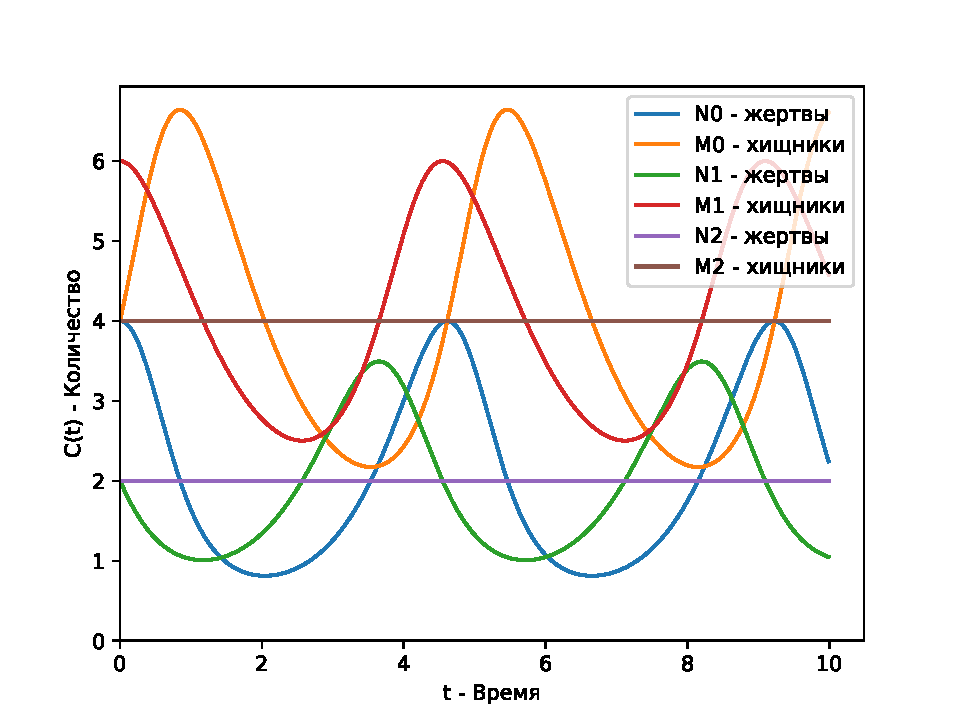
\includegraphics[width=11cm]{pictures/population.pdf}
            \caption{Графики при $a = 2, c = 0.5, b = 1, d = 0.5$, с начальными условиями $x_0=(4,4), ~ x_1 = (2,6), ~ x_2 = (N_e, M_e)$}
        \end{figure}

        \begin{figure}[H]
            \centering
            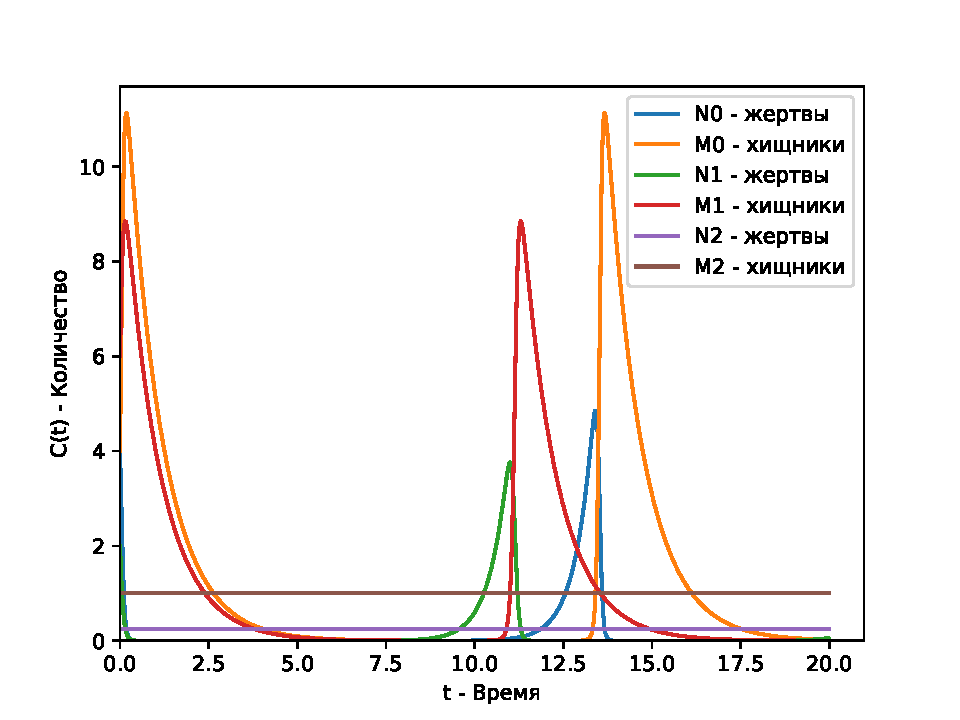
\includegraphics[width=11cm]{pictures/population2.pdf}
            \caption{Графики при $a = 2, c = 2, b = 1, d = 4$, с начальными условиями $x_0=(4,4), ~ x_1 = (2,6), ~ x_2 = (N_e, M_e)$}
        \end{figure}

    
    \subsection{Графики на фазовой плоскости}
        \begin{figure}[H]
            \centering
            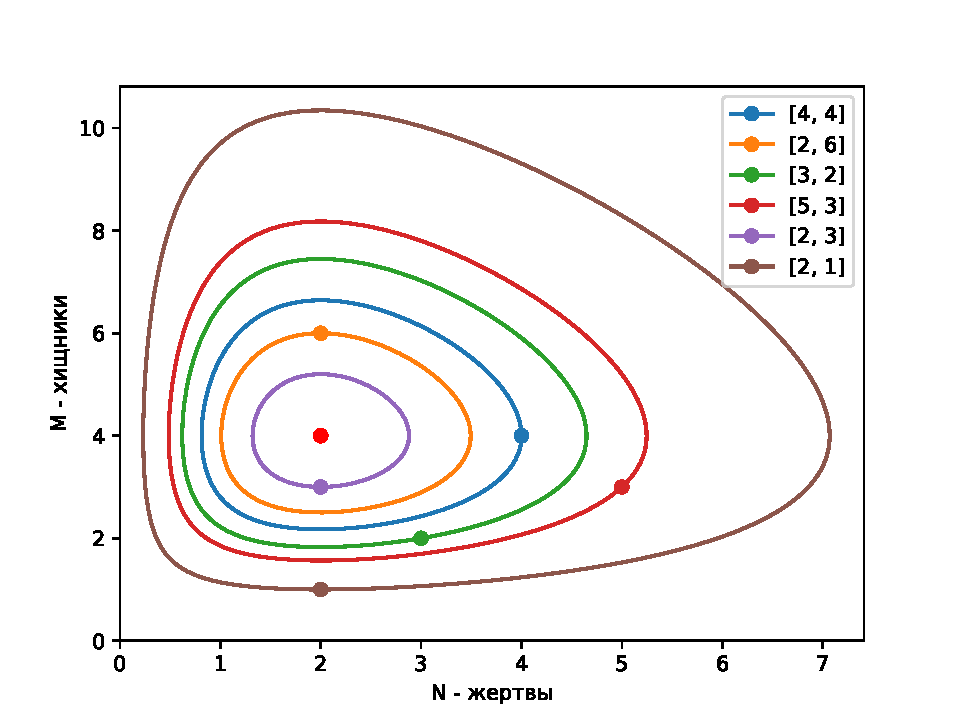
\includegraphics[width=12cm]{pictures/population3.pdf}
            \caption{Графики при $a = 2, c = 0.5, b = 1, d = 0.5$, с указанными начальными условиями на интервале времени $ [0, 10] $.}
        \end{figure}

        \begin{figure}[H]
            \centering
            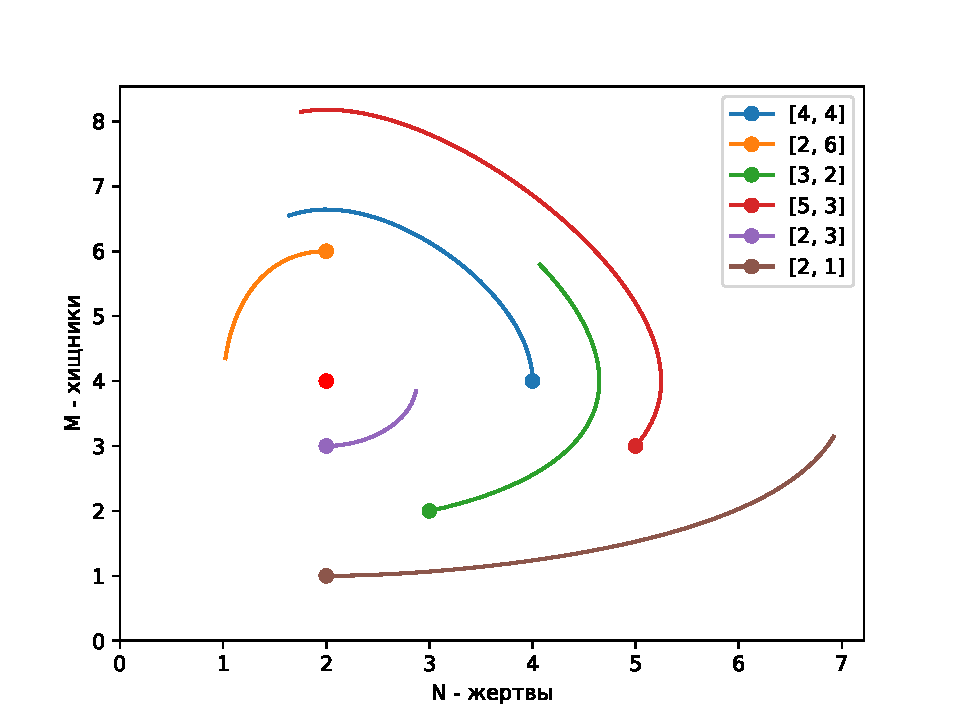
\includegraphics[width=12cm]{pictures/population4.pdf}
            \caption{Графики при $a = 2, c = 0.5, b = 1, d = 0.5$, с указанными начальными условиями на интервале времени $ [0, 1] $.}
        \end{figure}

        \begin{figure}[H]
            \centering
            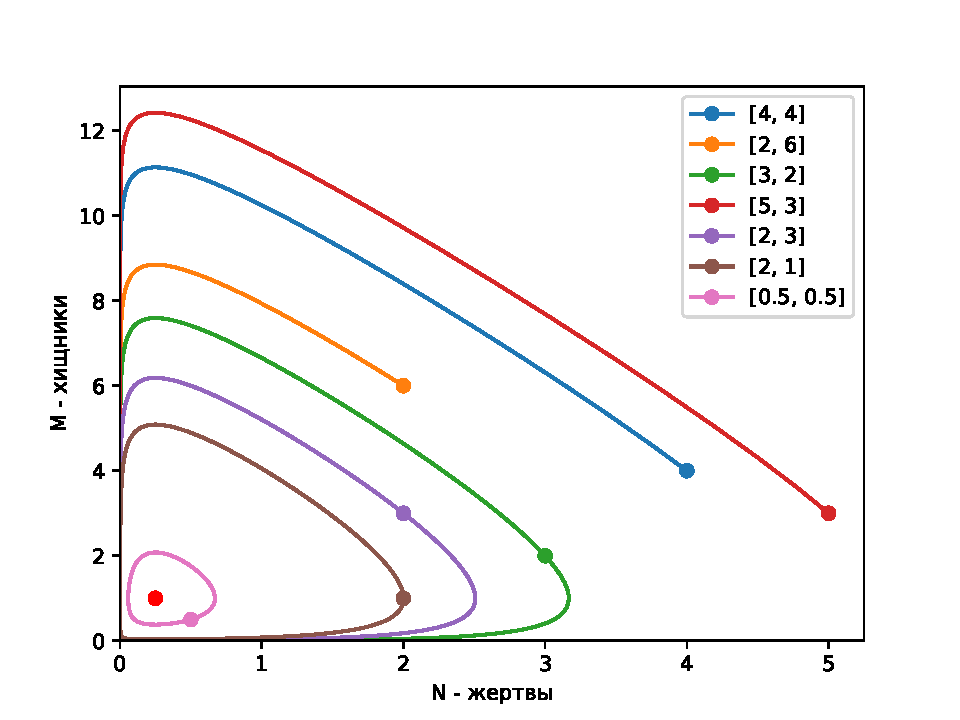
\includegraphics[width=12cm]{pictures/population5.pdf}
            \caption{Графики при $a = 2, c = 2, b = 1, d = 4$, с указанными начальными условиями на интервале времени $ [0, 10] $.}
        \end{figure}


